\documentclass{article}
\usepackage[utf8]{inputenc}
\usepackage{graphicx}
\usepackage{tikz}
\usepackage{todonotes}
\usepackage[hidelinks]{hyperref}
\usetikzlibrary{arrows, arrows.meta}
\usepackage{float}
\usepackage[]{algorithm2e}
\usepackage{pgfplots}
\usepackage{minted}

% Use standard A4 paper and standard margins for A4.
\usepackage[a4paper, margin=2.54cm]{geometry}

\begin{document}
\begin{titlepage}
    \begin{center}
       \vspace*{4cm}

       \textbf{\LARGE Tetris Project for AOS}

       \vspace{1.5cm}
        Design Document for the Tetris project for the course "Advanced Operating System".
            
       \vfill

       \textbf{Authors:}\\
       Accordi Gianmarco\\
       Chierici Franco

       \vspace{0.8cm}
     
       
\includegraphics[width=0.4\textwidth]{img/Logo_Politecnico_Milano.png}
            
       Dipartimento di Elettronica, Informazione e Bioingegneria\\
       Politecnico di Milano\\
       Italy\\
       29/03/2021
            
   \end{center}
\end{titlepage}

\tableofcontents

\newpage

\section{Introduction}
The aim of this document is to explain the design choices we have have made during the development of our project: a version of Tetris working from a terminal console, that is executed on an external microcontroller integrated circuit. 
It will also contain all the references to better understand the structure of the code.

\section{Design}

\subsection{Interfaces Diagram}
\begin{figure}[H]
    \centering
    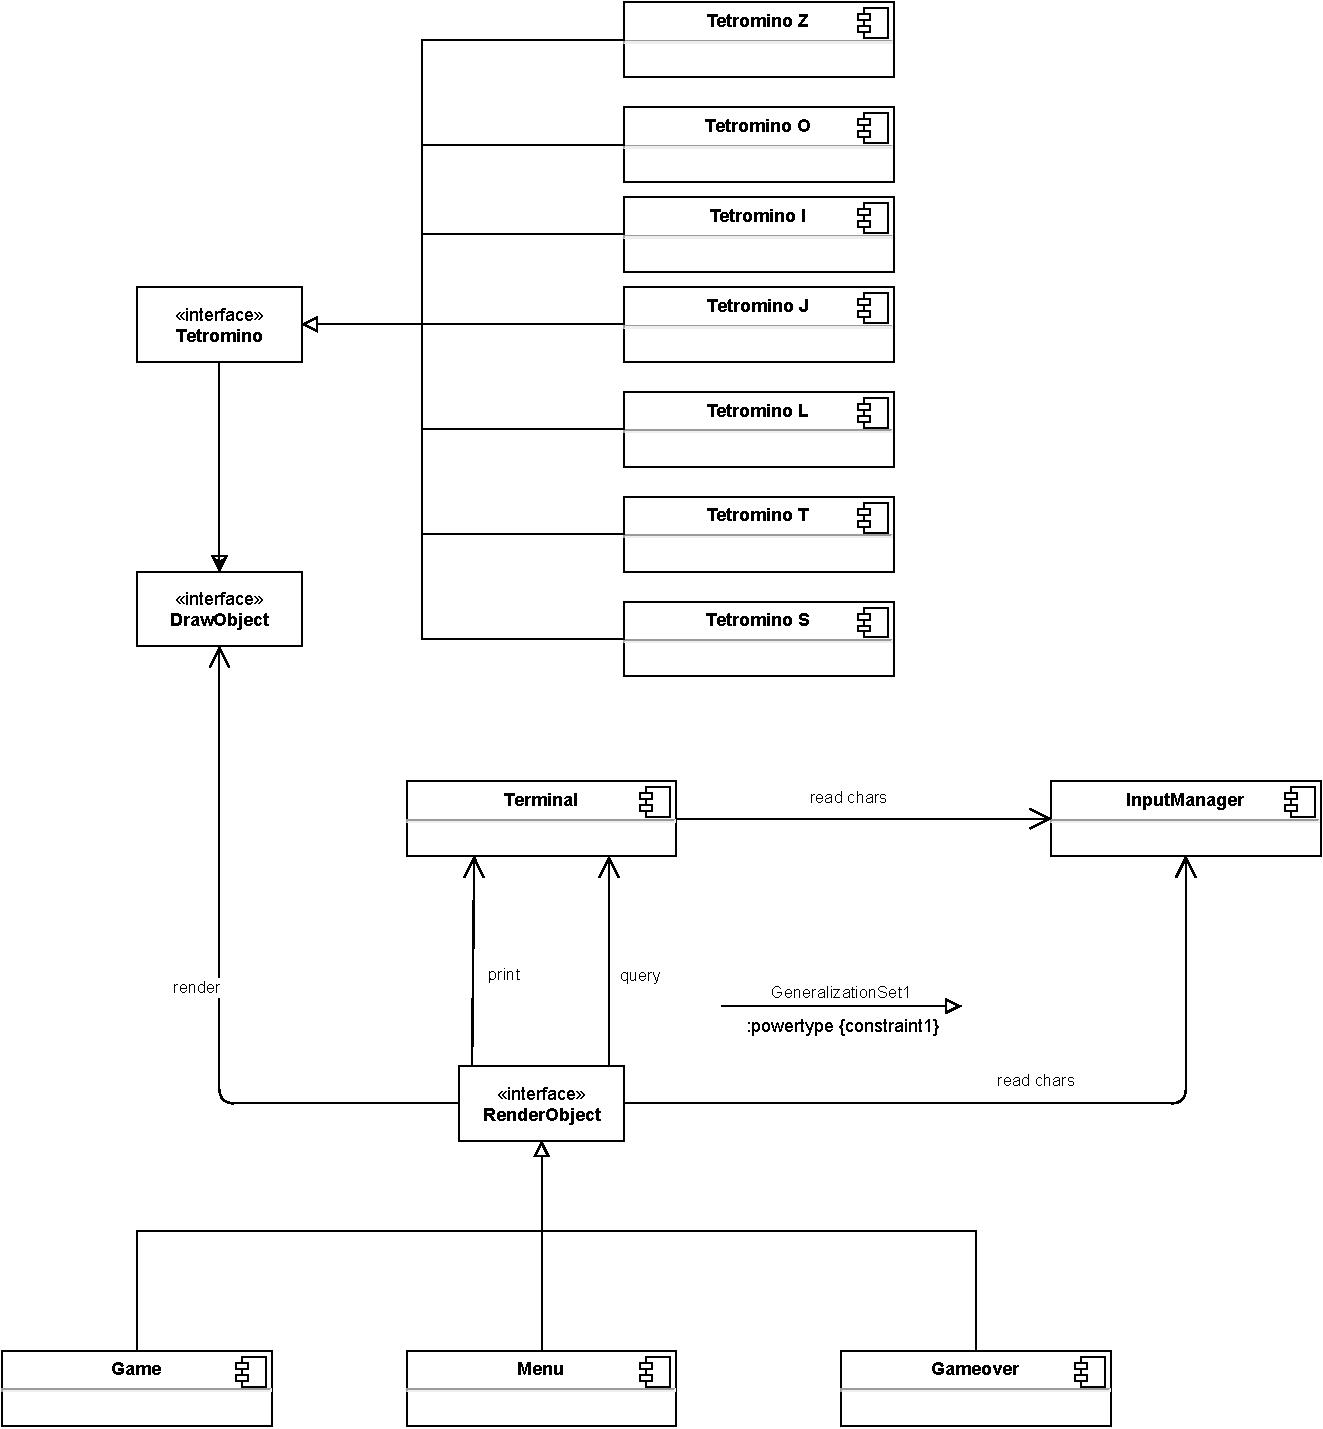
\includegraphics[width=\linewidth]{img/InterafcesDiagram.pdf}
    \caption{Interfaces Diagram of the project.}
    \label{fig:interface}
\end{figure}
The previous diagram \ref{fig:interface} shows the high level structure of the project. From it you can see that there are two relevant classes: the \textit{Terminal} and the \textit{InputManager}.
They are two implementation dependent classes that have been introduced in order to decouple the main project logics from the actual platform used.
The \textbf{Terminal} class is used to query the terminal to get the available space on the terminal screen, to set the terminal mode, and to print object on it, as further detailed inside \ref{terminal-rendering}.
When needed, the following functions are exposed by the Terminal:
\begin{minted}[linenos, bgcolor=white, escapeinside=!!]{c++}
    /* When needed use this method to update the value of col and row */
    int refreshColAndRow();
    /* Set the position of the cursor to the left higher corner of the drawing area, relative
    to the given row and col. */
    void positionCursorForStartDrawing(int posRow, int posCol);
    /* Draw a portion of the screen based on DrawObject
    starting from the position on screen (writingRow, writingCol). */
    void drawOnScreen(DrawObject drawObject, int writingRow, int writingCol);
\end{minted}
The Terminal class is instantiated in the entry point of the project that is obviously located at \path{main.cpp}, along with the declaration of the InputManager, then the references on top of them are carried along and passed in the constructor of each
element that is interested.
The \textbf{InputManager} instead manages the interactions with the user, it collects the characters received from the user in a queue, that is later on read by interested elements (like a \textit{RenderObject}).
\begin{minted}[linenos, bgcolor=white, escapeinside=!!]{c++}
    /* Returns an instance of the last char received from the user.
    NOTE: it is a blocking call. */
    char getLastChar();
    /* Returns an instance of the last char received for the terminal.
    NOTE: it is a blocking call. */
    char getLastCharForTerminal();
\end{minted}
It keeps track of two different queues: one that can be accessed by each element, and the second one only by the terminal. Since we are using ASCII Escape Sequence, we will query the terminal and receive response on the STDIN, so when doing this operation we suspend the adding into the queue of the next char on the STDIN,
and instead we put these chars on the queue for the Terminal. In this way we avoid that the two different streams of chars are mixed altogether.
One of the other Main interfaces is the \textbf{RenderObject}. There will be only one RenderObject at a time, and will be managed by the main code.
As detailed in the \ref{main-loop} each frame we draw is done by calling on the active RenderObject the method:
\begin{minted}[linenos, bgcolor=white, escapeinside=!!]{c++}
    /* Render method of the screen through the Terminal. */
    virtual RenderObject * drawFrame();
\end{minted}
Each draw action will be done by the Terminal, and sometimes this action requires either the whole content of the screen to be cleared (and so a call to \textit{resetScreen()} on Terminal is done), or only a portion of it (by using \textit{revertDrawObject()} to undone a previous print, this is done in order to reduce the number of transferred characters).
The various RenderObject are: \textit{Game}, \textit{Menu}, and \textit{Gameover}.
They all contain the logic used to implement the game.
The other abstraction we have made is to define the \textbf{DrawObject}, that is an object composed by the following fields:
\begin{minted}[linenos, bgcolor=white, escapeinside=!!]{c++}
    /* Is the string associate to this DrawObject */
    string object_string;
    /* Is the color associate to this DrawObject */
    string color;
\end{minted}
These fields are used by the Terminal when a call to print a DrawObject is done.
The last level of abstraction is represented by the \textbf{Tetromino}, that provides a high level interface, that is extended for every other Tetromino. In this way, each new Tetromino implementation we need requires only to provide a valid constructor, that draws the shape of the Tetromino as it was drawn on a Grid.
In fact, also the state of the game inside the \textbf{Game} class is saved inside a grid, then when needed is translated into a DrawObject and sent to the Terminal to be printed.
The definition of the Tetromino class includes also:
\begin{minted}[linenos, bgcolor=white, escapeinside=!!]{c++}
    /* Returns a string that should be printed on screen. */
    DrawObject toDrawObject();
\end{minted}
that is used in order to get the DrawObject starting from the Tetromino that should be sent to the Terminal to be printed.

\subsection{Sequence Diagram}
\begin{figure}[H]
    \centering
    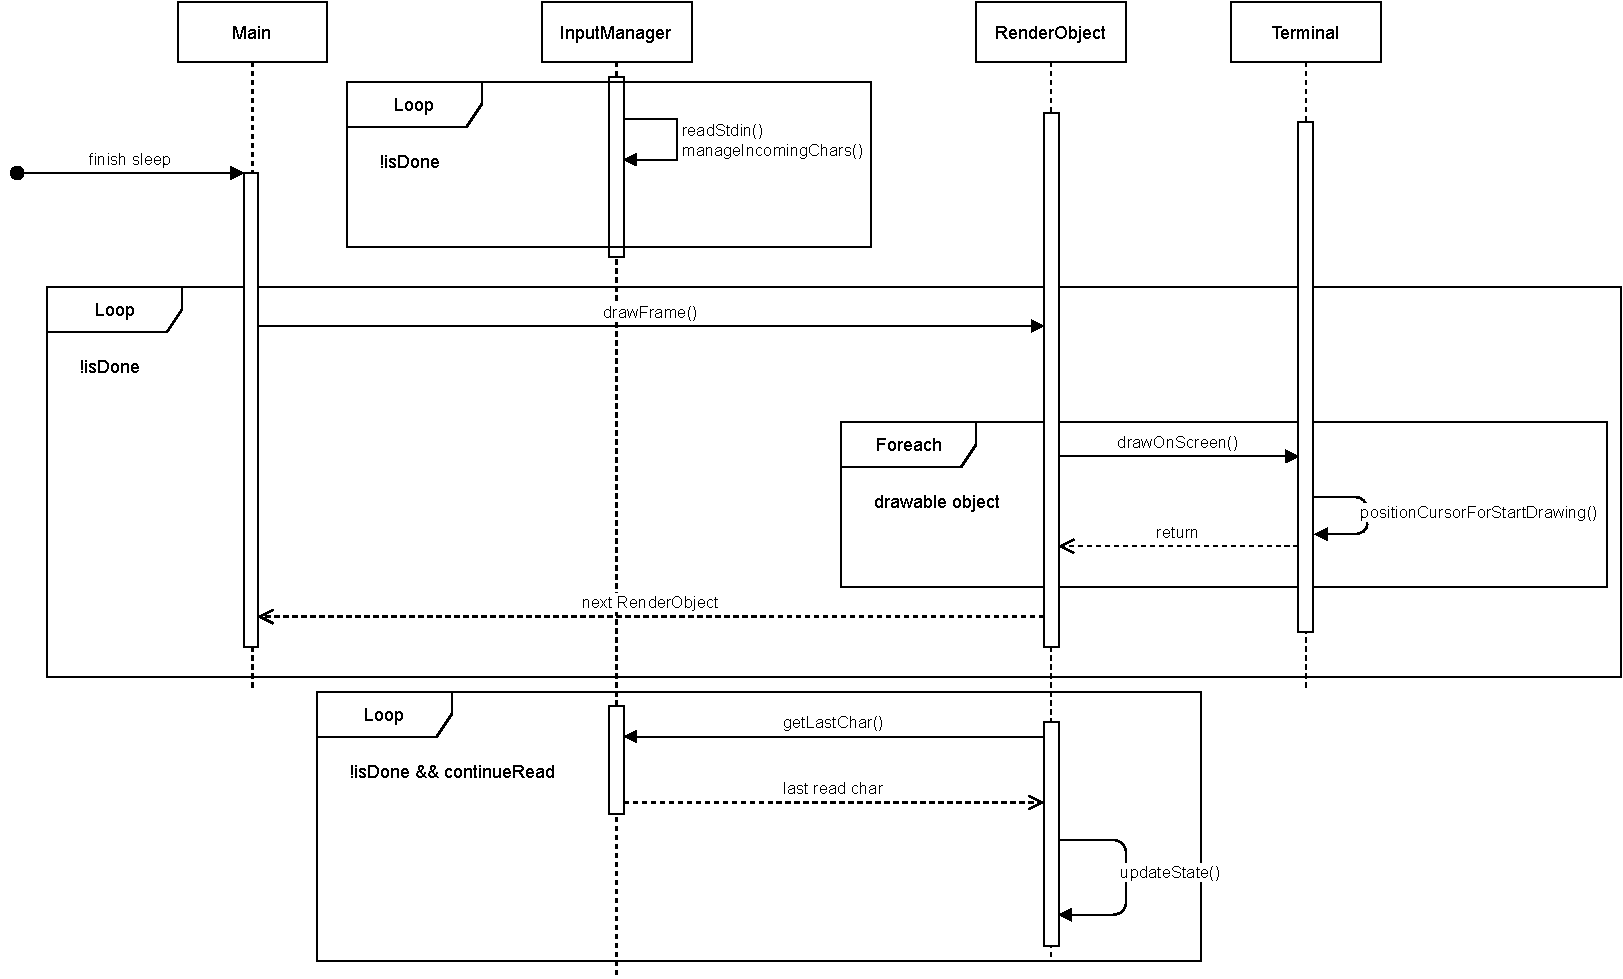
\includegraphics[width=\linewidth]{img/SequenceDiagram.pdf}
    \caption{Sequence Diagram of the project.}
    \label{fig:sequence}
\end{figure}
The above figure better explains how the components interact among them, and the interactions with the user.
First of all, since we will have different threads that have to coordinate among them, we have defined a global variable inside \path{terminal/utility.h}:
\begin{minted}[linenos, bgcolor=white, escapeinside=!!]{c++}
    extern atomic<bool> isDone;
\end{minted}
That has the scope to signal to the threads when to terminate the computation: for example, when the user presses the quit key, every thread is shut down correctly. Also, the access to the variable is made sequential thanks to the usage of the atomic type.
As said, we have adopted a multi-threaded architecture:
\begin{itemize}
    \item the \textbf{InputManager} class has a thread that reads the chars on the stdin and puts them in the correct queue;
    \item the \textbf{RenderObject} instead has a thread that is used in order to read the chars inside the interested queue from the InputManager, and then calls the \textit{updateState()} method to update the state of the object based on the received char. It is modeled like a finite state machine;
    \item \textbf{Game} has a thread that has to update the state of the Tetrominos used in the game, for example by making a Tetromino sliding down as time passes.
\end{itemize}
The figure also highlights three of the main interactions that happen between these components.
For example the first loop is the one of the thread on the InputManager that reads the char from the STDIN;
The second loop is a series of invocations that starting from the main, makes the call to draw the frame based on the current active RenderObject, that will draw the DrawObject associated to the current state.
At the end the active RenderObject will return a new RenderObject different from NULL, if we have to change the scene, for example when from the Menu the user starts a Game.
The third loop is instead the interaction between the InputManager and the other components interested in getting the last chars from the queues. In fact, we have defined two queues, one for the chars that are of interest to the RenderObjects and the other for the Terminal.
Moreover, in the file \path{miosix/config/arch/cortexM4_stm32l4/stm32l476rg_nucleo/board_settings.h}:
\begin{minted}[linenos, bgcolor=white, escapeinside=!!]{c++}
    const unsigned int defaultSerialSpeed=115200;
\end{minted}
we have changed the value of the Band Rate from 19200 to 115200. In this way, the drawing of a scene is done more quickly, since the characters exchange between the board and the PC is faster.

\section{Target Platform}
Since we have used as target the miosix-kernel, the supported boards are those officialy supported by the kernel itself. We have done most of our work on the STM32 Nucleo-64\footnote{https://www.st.com/en/evaluation-tools/nucleo-l476rg.html}.

\section{Implementation}
This part of the document better highlights how we have proceeded in the implementation of our project starting from the design, in a more technical perspective.

\subsection{Packages}
Our project has been developed by using C++\cite{slidec++}, in order to be compliant with the miosix-kernel\cite{miosix}.
We choose C++ over C because we found very useful the object-oriented paradigm. 

\subsubsection{Miosix}
This OS kernel allowed us to abstract from bare-metal programming, and made the management of multithreading easier\cite{slidebaremetal}\cite{osprogramming}.
\subsubsection{GDB}
The debugger helped us to find bugs and load the program into the board. Also, with the file \emph{.gdbinit} we have automated the debug process, that consists of connecting to the debug server and loading of the \emph{main.bin} into the board for execution.
\subsubsection{Screen}
Screen is a terminal multiplexer, that allows the board to use a remote terminal session, in this case Ubuntu's terminal, so that the user gets a UI for interfacing with the board and play Tetris.
 
\subsection{Terminal Rendering}
\label{terminal-rendering}
To render the frames, the first thing we did was to change the terminal mode. Usually it is set in canonical mode, where the program receives the input only when the user presses enter.
To achieve a "raw mode", thanks to the library \textit{Termios}, we turned off the local flag ICANON, that sets the terminal to canonical mode, and the ECHO flag.
The ECHO flag tells the terminal to print every key that the user is writing, and by default it is on, because normally users want to see what they are typing.
In order to get the terminal size, to reset the screen, to change the cursor position, and to make a colorful UI, we have used the ANSII Escape Sequences\footnote{https://en.wikipedia.org/wiki/ANSI\_escape\_code}. 

\subsection{Main Loop}
\label{main-loop}
\begin{algorithm}[H]
    Setup of the InputManager and the Terminal\;
    \While{!isDone} {\
        Call drawFrame() on the actualRenderObject\;
        \If{the returnedRenderObject!=NULL}{
            update actualRenderObject with the returnedRenderObject\;      
        }
        Sleep for 500 milliseconds\;
    }
\end{algorithm}
This is the loop executed in the main, that draws a frame every 500ms, thanks to the last sleep.
It maintains updated the actualRenderObject based on the value returned by the RenderObject upon updating the scene.
After rendering the scene in the last frame, the main awaits for 500 milliseconds, and it stops its computation if someone has updated the value of isDone to true, for example if the user has pressed the quit key.
Another important part is how the user input is managed inside the InputManager:\newline
\begin{algorithm}[H]
    \While{!isDone} {\
        get last char\;
        manage the incoming char\;
    }
\end{algorithm}
The second line of the pseudocode of particular interest, based on the state of the variable:
\begin{minted}[linenos, bgcolor=white, escapeinside=!!]{c++} 
    atomic<bool> awaitSequenceForTerminal;
\end{minted}
If it is true, it means that the Terminal class has recently queried the terminal with the ANSII Escape Sequence, and it is still in waiting for all the requested chars to be printed on the STDIN, taken by the InputManager and then stored inside 
\begin{minted}[linenos, bgcolor=white, escapeinside=!!]{c++}
    queue<char> lastCharsForTerminal;
\end{minted}
All other chars instead finish inside
\begin{minted}[linenos, bgcolor=white, escapeinside=!!]{c++}
    queue<char> lastChars;
\end{minted}
The last important piece of computation of interest is the work done by the thread associated with each RenderObject:\newline
\begin{algorithm}[H]
    \While{isDone AND continueRead)} {\
        get last char from the input manager queue of chars\;
        update the RenderObject state based on the char read from the queue\;
    }
\end{algorithm}
The update state part is used to separate the part of state update to the one of rendering, in this way we updated the state only based on the user input, while instead when a frame is rendered, the state is not changed, and the drawn scene will reflect the previous updates.

\subsection{Development Note}
In order to proceed with the development of our project, we have locally cloned the github repository of the miosix kernel\footnote{https://github.com/fedetft/miosix-kernel}.
After removing the \emph{.git} folder, we have also cloned into the same folder our repository\footnote{https://github.com/gianfi12/AOS-Tetris}.
In order to keep our code as parametric as possible, we have defined a header file at \path{terminal/utility.h} that acts as a configuration file.

\section{Target Platform}
Our board is the \emph{NUCLEO-L476RG}, it has a mini-USB controller, 1 LED, 1 user and 1 reset push-buttons, 76 pins.
It is provided with 1 Mbyte of flash memory, 128 Kbytes of SRAM, and a 80 MHz Arm Cortex-M4 core.

\section{Setup and Usage}
First, it is necessary to clone the repository of the miosix kernel\footnote{https://github.com/fedetft/miosix-kernel}, and remove the relative\emph{.git} folder.\newline
Then, clone into the same folder our repository\footnote{https://github.com/gianfi12/AOS-Tetris}.\newline
To configure the miosix kernel, follow the Getting Started section in the Miosix Wiki page\footnote{https://miosix.org/wiki/index.php?title=Quick\_start\#Getting\_started} 
and the In-circuit debugger section\footnote{https://miosix.org/wiki/index.php?title=Quick\_start\#In-circuit\_debugger}.\newline

After that, plug in the board, in our case the STM32 Nucleo-64, open the terminal in the miosix-kernel directory and run the command
\begin{minted}[linenos, bgcolor=white, escapeinside=!!]{bash}
    openocd -f stm32l4nucleo.cfg
\end{minted}
in order to open the communication between the board and the computer.\newline
Now, open a new terminal and run
\begin{minted}[linenos, bgcolor=white, escapeinside=!!]{bash}
    screen /dev/ttyACM0 115200
\end{minted}
This is where the board will write on the screen. Note that if the size of this terminal is less than 65x45, the program will print an error and close.
Then, in a new tab of the terminal, again in the directory miosix-kernel, run the command
\begin{minted}[linenos, bgcolor=white, escapeinside=!!]{bash}
    arm-miosix-eabi-gdb main.elf
\end{minted}
if you want to debug it with gdb. If you have defined as present in the folder the .gdbinit file, the process of connecting to the debug server and the load of the program is automated.

Finally it is time to play Tetris! Press enter to start the game and q to exit.
Use the arrows to move left, right or down the Tetromino. Press A to rotate the Tetromino counterclockwise, S to move it clockwise.
When you fill an entire row, it will be canceled and your score will be updated.\newline
If you manage to fill 4 rows, congratulations, you just made Tetris!\newpage

\section{Results}
These are the screenshots of the game.

\begin{figure}[H]
    \centering
    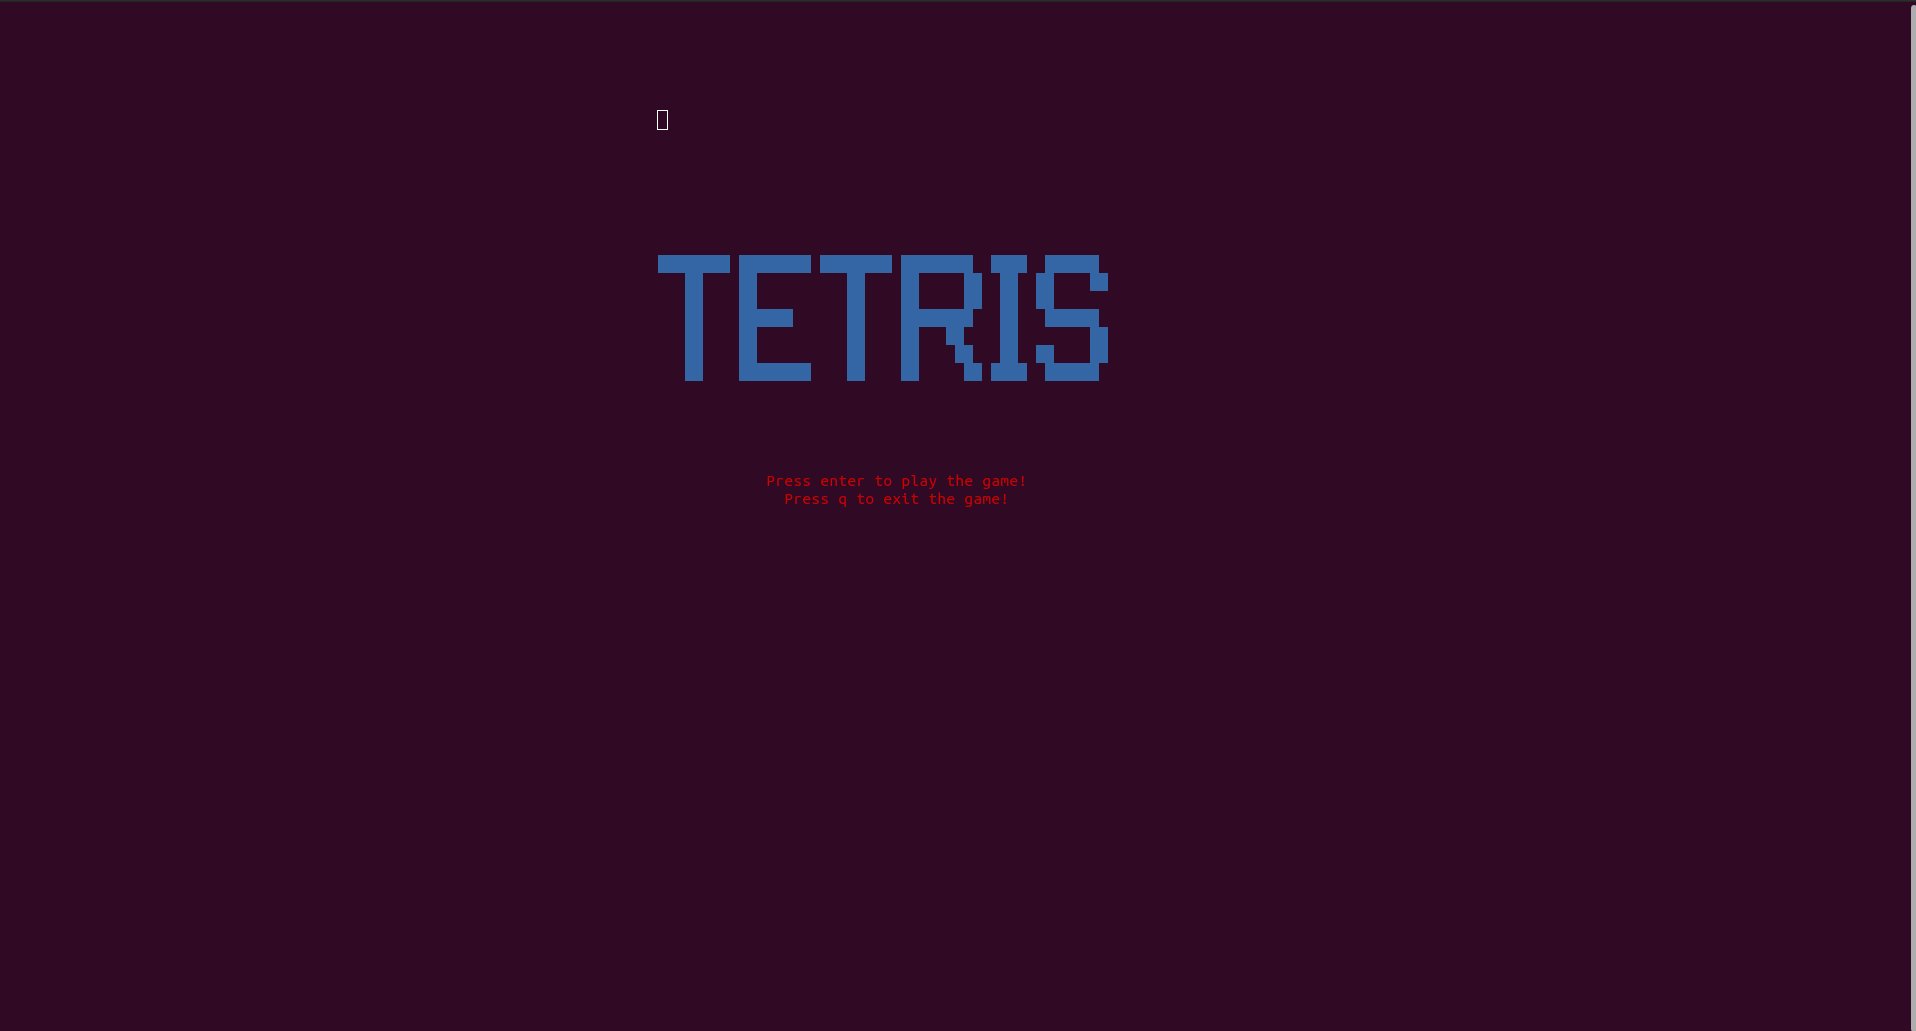
\includegraphics[width=\linewidth]{img/in_game/Tetris_home.png}
    \caption{Home screen of the game}
    \label{fig:home_screen}
\end{figure}

\begin{figure}[H]
    \centering
    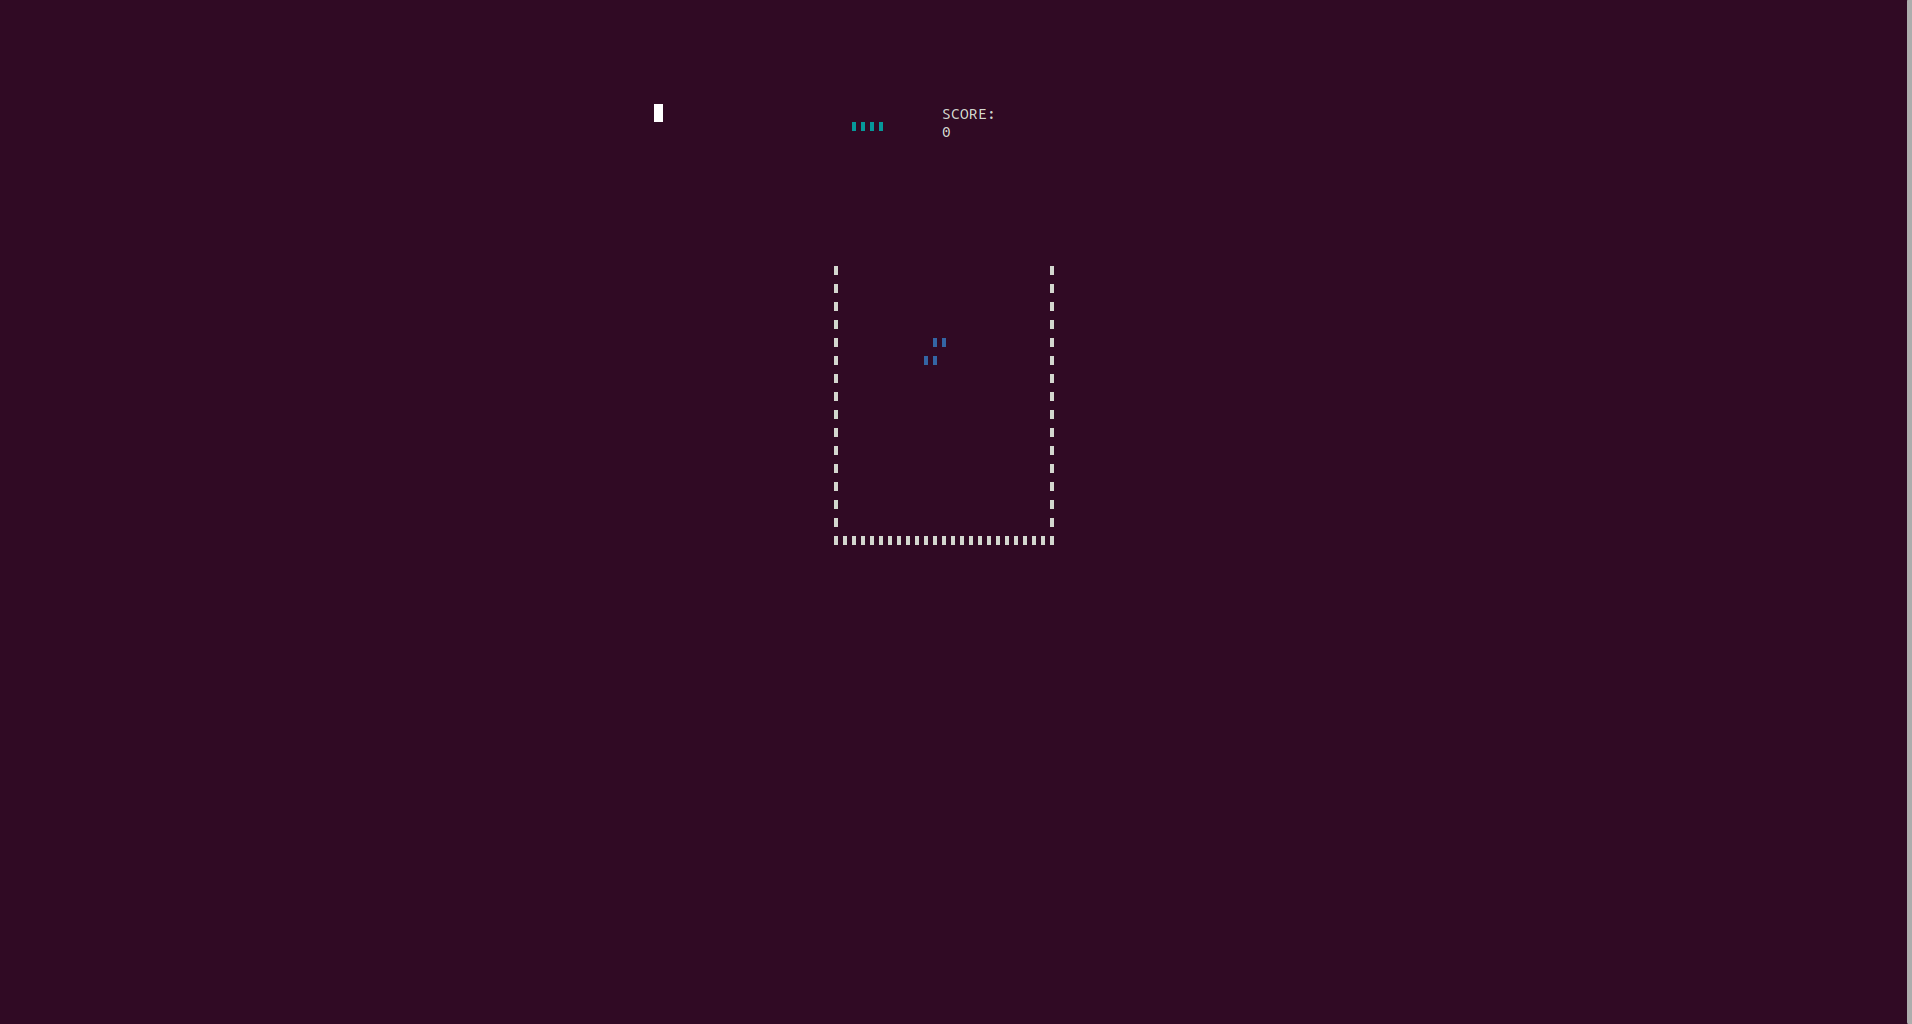
\includegraphics[width=\linewidth]{img/in_game/Tetris_game_started.png}
    \caption{In-game graphics (1)}
    \label{fig:game_started}
\end{figure}

\begin{figure}[H]
    \centering
    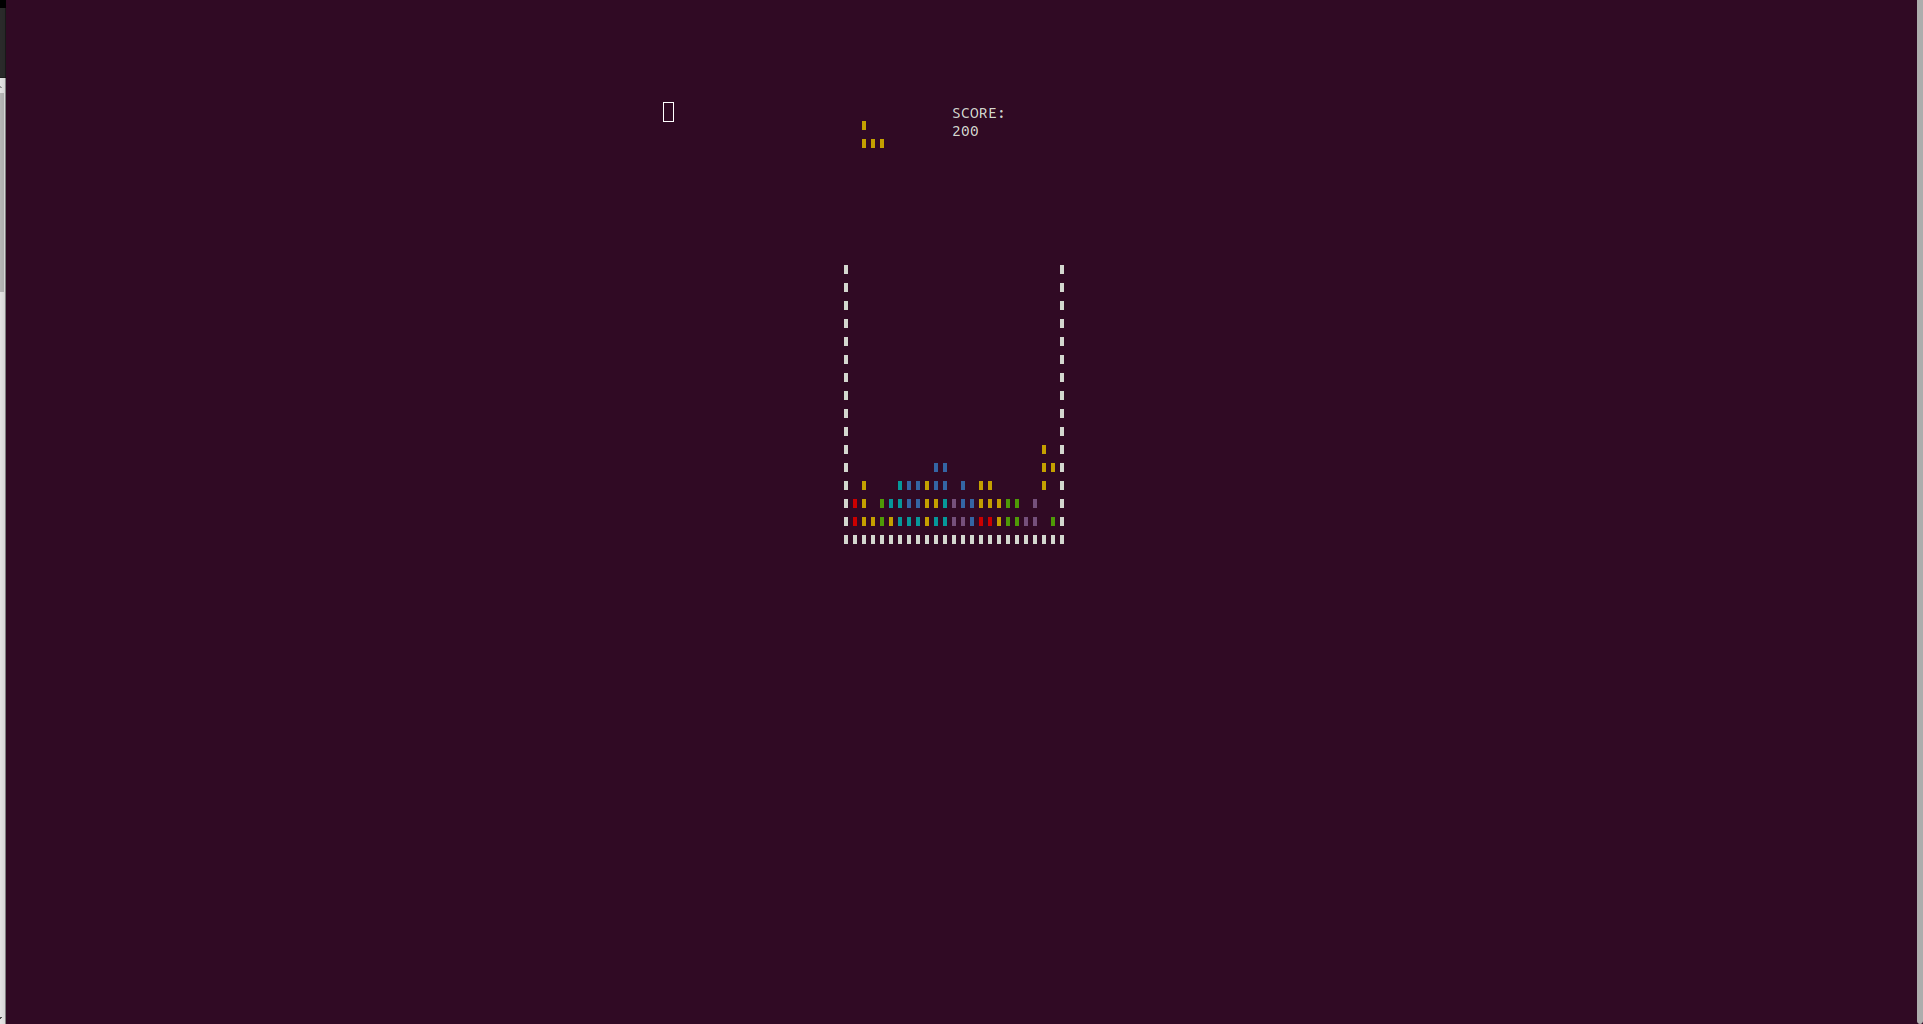
\includegraphics[width=\linewidth]{img/in_game/Tetris_mid_game.png}
    \caption{In-game graphics (2)}
    \label{fig:mid_game}
\end{figure}

\begin{figure}[H]
    \centering
    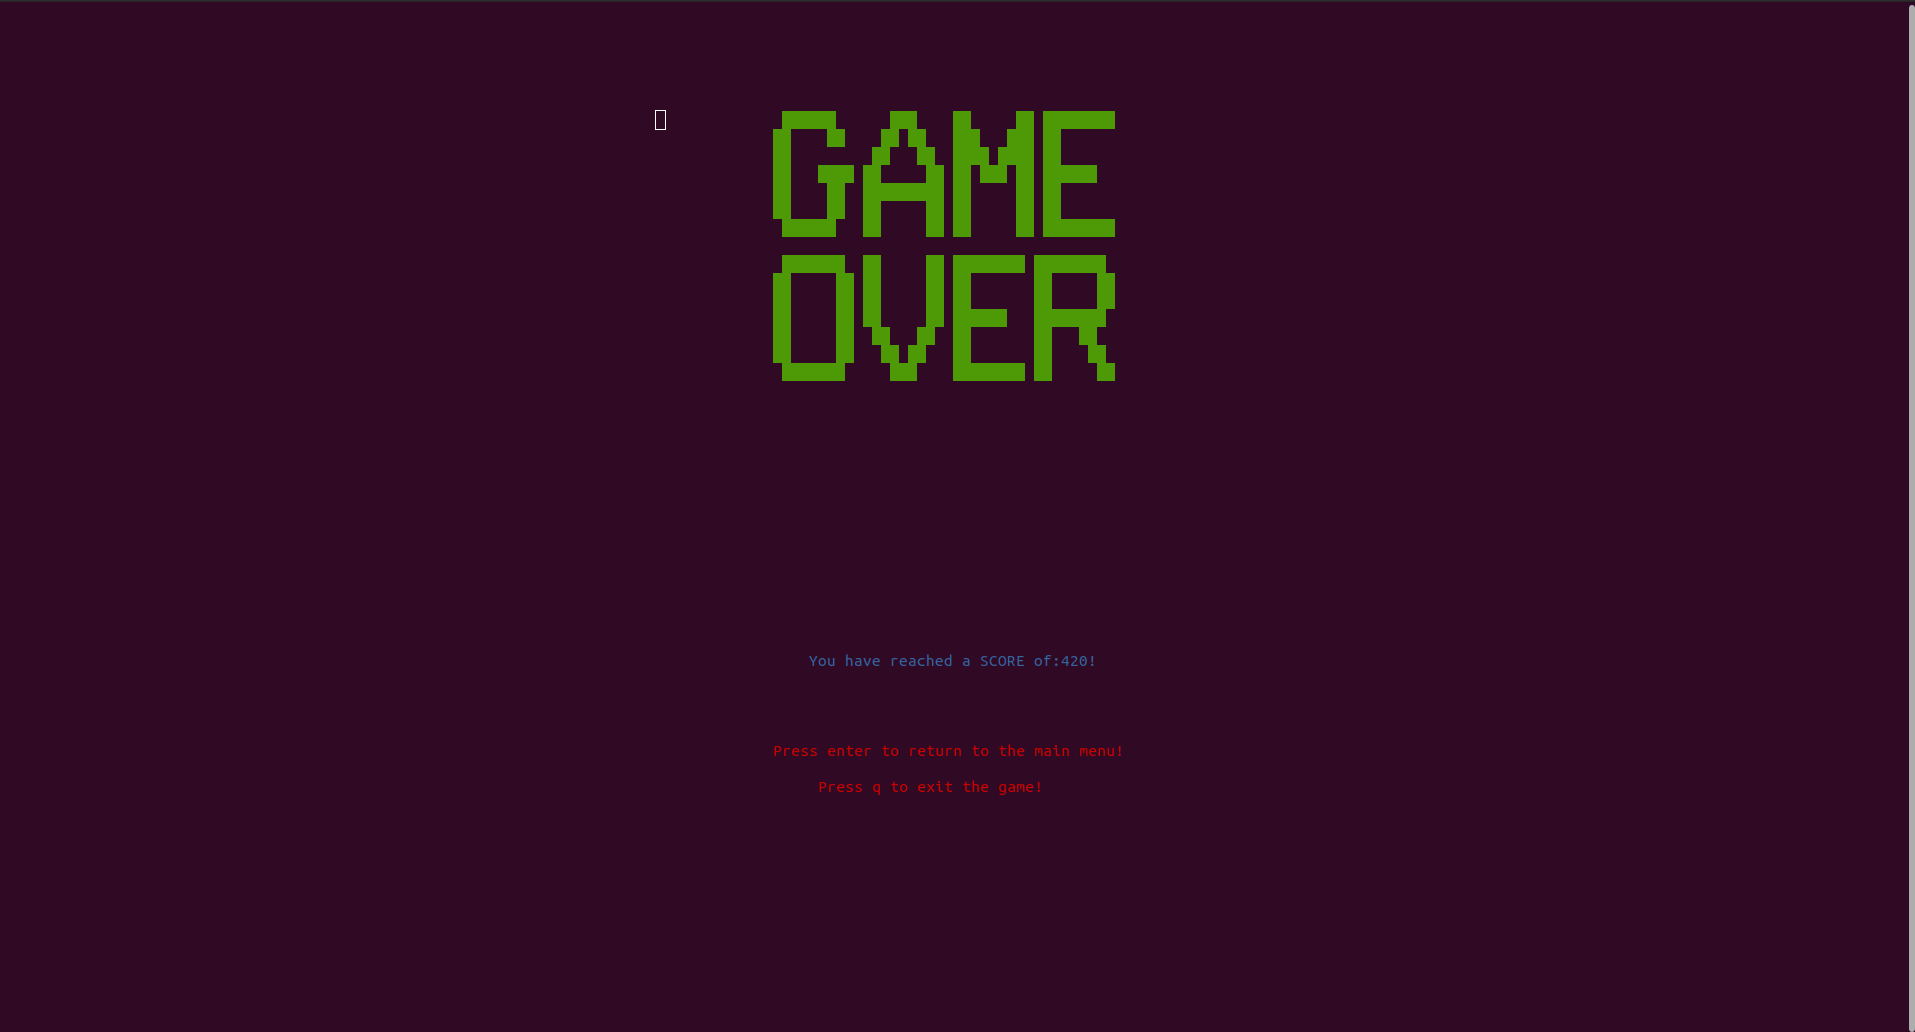
\includegraphics[width=\linewidth]{img/in_game/Tetris_game_over.png}
    \caption{Game over screen}
    \label{fig:game_over}
\end{figure}

\begin{figure}[H]
    \centering
    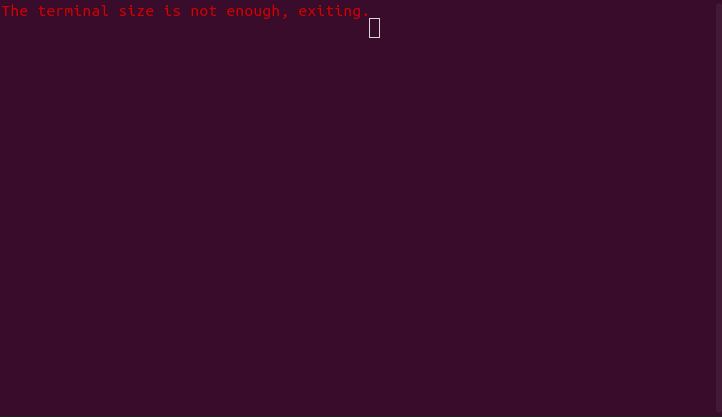
\includegraphics[width=\linewidth]{img/in_game/Tetris_error.png}
    \caption{Error screen (terminal too small)}
    \label{fig:termial_size_error}
\end{figure}

\bibliographystyle{plain}
\bibliography{references}
\end{document}